\documentclass[a4paper, 11pt]{article}

\usepackage{graphicx}
\usepackage{graphics}
\usepackage{verbatim}
\usepackage{listings}
\usepackage{color}

\begin{document}

\title{Report: hierarchical workstealing in XKAAPI}
\author{XKAAPI team}
\date{}

\maketitle

\newpage
\tableofcontents
\addtocontents{toc}{\protect\setcounter{tocdepth}{1}}

% \part{title}
% \section{title}
% \subsection{title}


% Introduction
%
\newpage
\section{Introduction}
\paragraph{}
TODO: describe the need for HWS


% Building and running
%
\newpage
\section{Enabling HWS in XKAAPI}

\subsection{Build configuration}
\paragraph{}
No new configuration has been added to the build system. However, the
runtime has to be compiled with \textit{hwloc} and \textit{numa} support
for HWS to be enabled:\\
\begin{small}
\begin{lstlisting}[frame=tb]
./configure --with-hwloc --with-numa
\end{lstlisting}
\end{small}

\subsection{Environment variables}
\paragraph{}
The steal request emission routine has to be specialized by setting the
\textit{KAAPI\_EMITSTEAL} environment variable to ``hws'':\\
\begin{small}
\begin{lstlisting}[frame=tb]
$> KAAPI_HWS_LEVEL=hws ./a.out
\end{lstlisting}
\end{small}

\paragraph{}
Specific memory heriarchy levels can be used by setting the
\textit{KAAPI\_HWS\_LEVELS} environment variable. It consists of a comma
separated list of one or more of the following values:
\begin{itemize}
  \item ALL: enables all the levels,
  \item NONE: disables all the levels,
  \item L3: enable the L3 cache level,
  \item NUMA: enable the numa level,
  \item SOCKET: enable the socket level,
  \item MACHINE: enable the machine level,
  \item FLAT: enable the flat level.
\end{itemize}
For instance:\\
\begin{small}
\begin{lstlisting}[frame=tb]
$> KAAPI_HWS_LEVEL=hws KAAPI_HWS_LEVELS=FLAT,NUMA ./a.out
\end{lstlisting}
\end{small}

\paragraph{}
Not setting this variable enables the NUMA, SOCKET, MACHINE and FLAT
memory levels.

% Implementation
%
\newpage
\section{HWS implementation in XKAAPI}

\subsection{Overview}
\paragraph{}
The \textit{src/hws} directory has been added to the runtime sourcecode. It implements:
\begin{itemize}
\item subsystem initialization (\textit{kaapi\_hws\_initialize.c}),
\item task pushing (\textit{kaapi\_hws\_pushtask.c}),
\item steal request emission (\textit{kaapi\_hws\_emitsteal.c}),
\item workstealing queue implementation (\textit{kaapi\_ws\_queue\_xxx.c}),
\item related performance counters (\textit{kaapi\_hws\_counters.c}),
\item scheduler synchronization (\textit{kaapi\_hws\_sched\_sync.c}) .
\end{itemize}

\subsection{Hierarchy construction}
\paragraph{}
TODO
\begin{figure}[!hb]
\centering
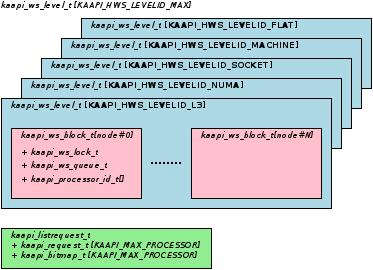
\includegraphics[keepaspectratio=true, scale=0.6]{../dia/impl/main.jpeg}
\caption{HWS data structure relations}
\label{hws_impl}
\end{figure}

\subsection{Steal request emission algorithm}
\paragraph{}
TODO

\subsection{Workstealing queue virtualization}
\paragraph{}
TODO

\subsection{Emisteal routine virtualization}
\paragraph{}
The \textit{emitsteal} routine has been virtualized. The
\textit{KAAPI\_EMITSTEAL} environment variable controls the
implementation used:
\begin{itemize}
\item hws: use the hierarhical workstealing implemented by the
\textit{kaapi\_hws\_sched\_emitsteal} routine,
\item any other value: use the default \textit{kaapi\_sched\_emitsteal} routine.
\end{itemize}


% Benchmarks
%
\newpage
\section{Benchmarks}
\paragraph{}
TODO


\end{document}
